\chapter{Applications}

\par
Les applications possibles à partir des cartes de saillance sont illimitées. Notre problématique ici était de réussir à \textbf{animer} nos peintures à partir de la carte de saillance générée par le modèle de saillance. Eakta Jain, professeur assistante à l'université de de Floride, a déjà travaillé avec Olivier et a pu nous apporter son expérience grâce aux différents projets d'applications basés sur le mouvement du regard qu'elle a réalisé \cite{eaktalab}. Ses projets liés au regard humain sont souvent appliqués aux comics qui a des similarités avec la peinture.

\section{Recherche d'application}

\par
Afin de déterminer quelle application il serait intéressant de développer, il faut faire une recherche de ce qui existe déjà ou inventer autre chose. Je vais présenter ici les différentes pistes qui ont été envisagées et expliquer notre choix final.

\par
Pour ajouter du mouvement, il existe des logiciels qui permettent de générer des \textbf{plotagraphes}. Basé sur les cinémagraphes, qui sont des mélanges d'images et de vidéos, les plotagraphes permettent d'ajouter du mouvement à partir de l'image seule. En revanche il faut ajuster à la main les zones à mouvoir donc difficilement automatisable et le résultat n'est impressionnant que sur les fluides (eau, nuages, fumée...).

\par
Eakta a un projet de \textbf{segmentation} des différentes parties d'un comic pour animer les personnes qui parle et ajouter du son \cite{segmentationcomics}. La segmentation est obtenue à partir du chemin visuel aquis par occulométrie. Une idée intéressante mais difficilement adaptable à toutes les peintures car trop détaillée.

\par
Un autre projet d'Eakta appelé "Predicting Moves-on-Stills for Comic Art using Viewer Gaze Data" \cite{kenburns} ajoute un effet de \textbf{Ken Burns} sur des pages de comics en fonction des prédictions du mouvement du regard du spectateur. Cet un effet intéressant et facile à mettre en place. C'est la piste vers laquelle on se dirigera et que l'on détaillera dans la partie suivante. Il existe aussi une version 3D de cet effet \cite{kenburns3D} qui est très impressionante mais est compliquée à mettre en place et difficile à mettre en relation avec la carte de saillance.

\newpage
\section{Effet Ken burns}

\par
L'effet \textbf{Ken Burns} est représenté par un mouvement de caméra (panoramique, zoom ou rotation) sur une image fixe. L'ajout de mouvement et d'animation permet de garder l'attention du spectateur. C'est un effet qui est très régulièrement utilisé dans les documentaires, dans les journeaux télévisés ou tout simplement dans les diaporamas photos. 

\begin{figure}[ht]
    \centering
    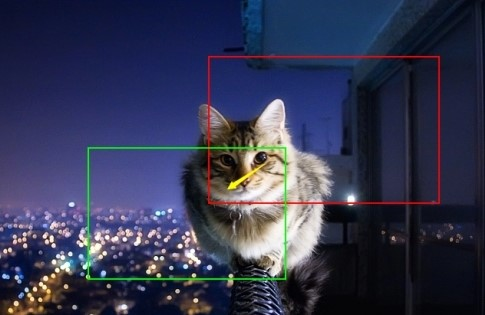
\includegraphics[width=0.7\linewidth]{datas/kenburnseffect.jpg}
    \caption{Exemple d'effet Ken Burns avec panoramique du cadre rouge vers le cadre vert}
    \label{kenburnsexemple}
\end{figure}

\par
J'ai donc décidé de partir sur un effet Ken Burns comme projet d'application. Mon but ici est que le mouvement de la caméra suive celui d'un \oe{}il humain. On est capable de généré un chemin visuel à partir d'une carte de saillance grâce à un \textbf{modèle saccadique}. J'ai pu en utiliser un créé par Olivier Le Meur \cite{saccadicmodel} disponible sur le gitlab de l'équipe Percept. Ainsi à partir d'une peinture on obtient une carte de saillance grâce au modèle de saillance, puis le chemin visuel grâce au modèle saccadique et enfin un effet Ken Burns qui suit le chemin visuel.

\par
Je me suis donc lancé dans la réalisation d'un programme en Python qui en entrée prend une peinture et le chemin visuel associé pour en sortie obtenir une vidéo avec l'effet Ken Burns. Le principe de base est d'avoir une caméra qui se déplace dans l'image et qui enregistre ses déplacements à la fréquence de la vidéo de sortie.

\par
J'ai décidé ici de faire le même schéma de déplacement pour chaque vidéo. Au début de la vidéo on a une pause sur la peinture entière pour que l'observateur puisse la voir dans son intégralité. Ensuite on fait un zoom x2 sur la première fixation de mon chemin visuel. Ensuite on fait des panoramiques pour passer d'une fixation à une autre. pour chaque fixation je fais une pause de quelques secondes pour que l'observateur puisse prendre le temps de regarder l'\oe uvre et d'identifier les petits détails. Enfin je fais un dézoom pour retrouver une vue d'ensemble de la peinture.

\par
Je me suis attaqué à la programmation des différents mouvements de caméra, le zoom et le panoramique. J'ai d'abord commencé par créer l'effet de zoom qui consiste à redimensionner l'image tout en gardant à l'identique la résolution de la caméra. Donc par exemple pour un zoom x2 je double la taille de l'image mais je garde celui de la caméra sur les dimensions d'origine. Une fois zoomé, le but est de se déplacer de fixation en fixation en suivant le chemin visuel. Afin d'obtenir des mouvements directs et de pouvoir gérer les bords proprement je précalcule la position finale de ma caméra puis je fais bouger la caméra de mon point d'origine vers la position finale. En fusionnant les deux mouvements on peut créer un zoom sur un point précis de l'image.

\par
Dans un premier temps le mouvement était trop linéaire ce qui a pour effet de donner un rendu final assez pauvre et saccadé. Pour lisser les mouvements j'ai appliqué un effet de ease-in-out. Cela permet d'obtenir une accélération progressive au début du mouvement et une décélération progressive à la fin. Au lieu d'avoir une interpolation linéaire (graphe \ref{subfig:lineaire}), c'est-à-dire que la caméra se déplace de la même distance entre chaque image d'un plan à un autre, ici on a une interpolation avec de petites distances en début et en fin de parcours mais de grandes distances en milieu de parcours (graphe \ref{subfig:ease}).

\begin{figure}[ht]
    \centering
    \begin{subfigure}{.49\textwidth}
        \centering
        \begin{tikzpicture}
            \begin{axis}[every axis plot post/.append style={
              mark=none,domain=0:60,samples=50,smooth},
                % All plots: from -2:2, 50 samples, smooth, no marks
              axis x line*=bottom, % no box around the plot, only x and y axis
              axis y line*=left, % the * suppresses the arrow tips
              enlargelimits=upper, % extend the axes a bit to the right and top
              ylabel=Coefficient,
              xlabel=Image]
              \addplot {x/60};
            \end{axis}
            \end{tikzpicture}
        \caption{Linéaire}
        \label{subfig:lineaire}
    \end{subfigure}
    \begin{subfigure}{.49\textwidth}
        \centering
        \begin{tikzpicture}
            \begin{axis}[every axis plot post/.append style={
              mark=none,domain=0:60,samples=50,smooth},
                % All plots: from -2:2, 50 samples, smooth, no marks
              axis x line*=bottom, % no box around the plot, only x and y axis
              axis y line*=left, % the * suppresses the arrow tips
              enlargelimits=upper, % extend the axes a bit to the right and top
              ylabel=Coefficient,
              xlabel=Image]
              \addplot {-(cos(pi*x)-1)/2};
            \end{axis}
            \end{tikzpicture}
        \caption{Ease-in-out}
        \label{subfig:ease}
    \end{subfigure}
    \caption{Graphes représentant les coefficients d'interpolations pour 60 images}
    \label{fig:graphes}
\end{figure}

\par
Et enfin comme les chemins visuels sont souvent composés d'une vingtaine de fixations souvent proches les unes des autres, j'ai décidé de ne pas faire un déplacement de caméra pour chacune d'enre elles. Cela ferait trop de répétition et perdrait le spectateur dans la peinture. A la place je fais en sorte que les fixations présentes sur un certain pourcentage du cadre de la caméra soit ignorées pour le reste du parcours de la caméra.

\section{Sous-titre descriptif}

\par
Pour améliorer l'application, Olivier, Eakta et moi avons pensé à un concept d'intelligence artificielle qui décrit ce qu'elle voit. L'idée ici serait d'ajouter aux vidéos des \textbf{sous-titres automatiques} générés par un réseau de neurones qui décrivent ce qui est représenté. Il en existe qui fonctionne pour des scènes naturelles avec par exemple le modèle Neuraltalk2 de Karpathy \cite{neuraltalk2} (\linkrename{lien démo}{http://cs.stanford.edu/people/karpathy/neuraltalk2/demo.html}).

\par
J'ai testé ce modèle sur les peintures mais le résultats est ridiculement mauvais. Quasiment aucune description ne correspond à l'image comme on peut le voir en exemple de l'image \ref{fig:ex_neuraltalk}. Il faudrait donc ré-entrainer le modèle pour pouvoir espérer obtenir de meilleurs résultats. Cependant plusieurs problèmes nous empêche de travailler sur cette solution. Premièrement le programme en lui-même est assez complexe et je n'ai pas réussi à faire tourner la partie entrainement du modèle. Deuxièmement il est très dur de modifié le dataset de mots puisque celui-ci est composé de mots associés à des éléments d'images que seul le modèle peut interprété. On a donc quasiment aucune maléabilité du dataset. Et troisièmement la fin du stage arrive trop vite pour que je prenne le temps de m'attarder dessus.

\begin{figure}[ht]
  \centering
  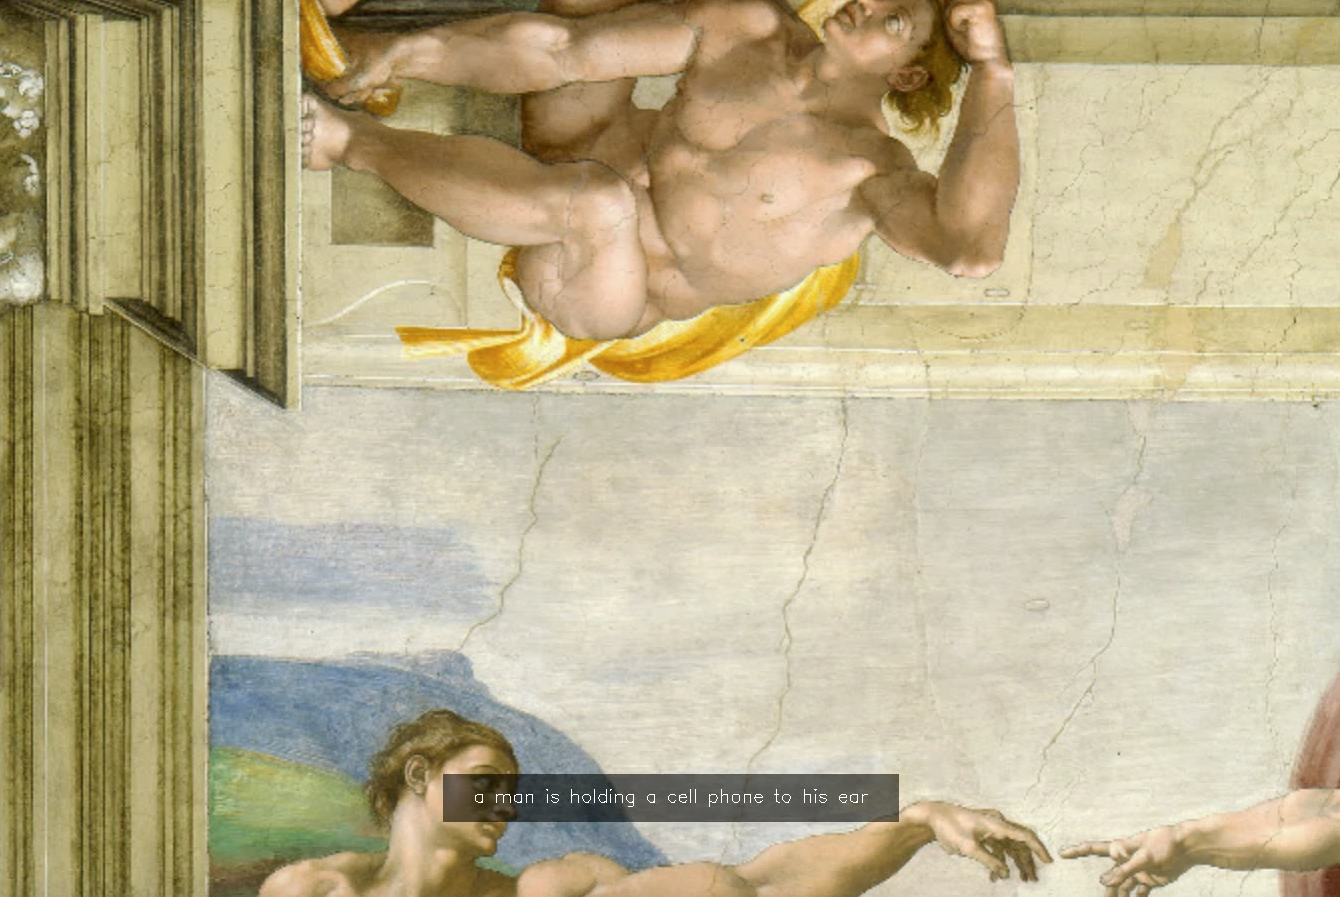
\includegraphics[width=0.7\linewidth]{datas/exemple_sous_titre.png}
  \caption{Exemple de sous-titre descriptif généré par Neuraltalk2 (\emph{Création d'Adam}, Michel-Ange, 1512)}
  \label{fig:ex_neuraltalk}
\end{figure}

\par
On a donc décidé avec Olivier de faire une \textbf{preuve de concept}. C'est-à-dire un script prototype qui permettrait de prouver qu'il est possible d'utiliser des sous-titres générés automatiquement sur ces peintures et des les intégrer à notre vidéo. J'ai donc modifié mon programme qui génère des vidéos pour pouvoir insérer du texte en bas de l'image. Cela m'as permis d'obtenir le résultat visible sur l'image \ref{fig:ex_neuraltalk}. Le programme de la preuve de concept se déroule en trois étapes. En premier je pré-génère les images lorsque la vidéo est en pause. Ensuite je rentre ces images dans le modèle de sous-titrage pour obtenir des images avec des descriptions. Enfin je génère la vidéo en ajoutant mes images sous-titrées lors des pauses de ma vidéo.

\par
Afin de pouvoir diffuser ces travaux sur les réseaux sociaux (LinkedIn ou Medium), j'ai ajouté à la pause du début de vidéo un sous-titre qui dit "What does an AI see in this paintings ?", traduit par "Que voit une IA dans cette peinture ?", ainsi que le nom de la peinture et de l'artiste en haut de la vidéo (voir image \ref{fig:title_screen}). Une question qui intrigue le spectateur et qui lui donne envie de regarder le reste de la vidéo.

\begin{figure}[ht]
  \centering
  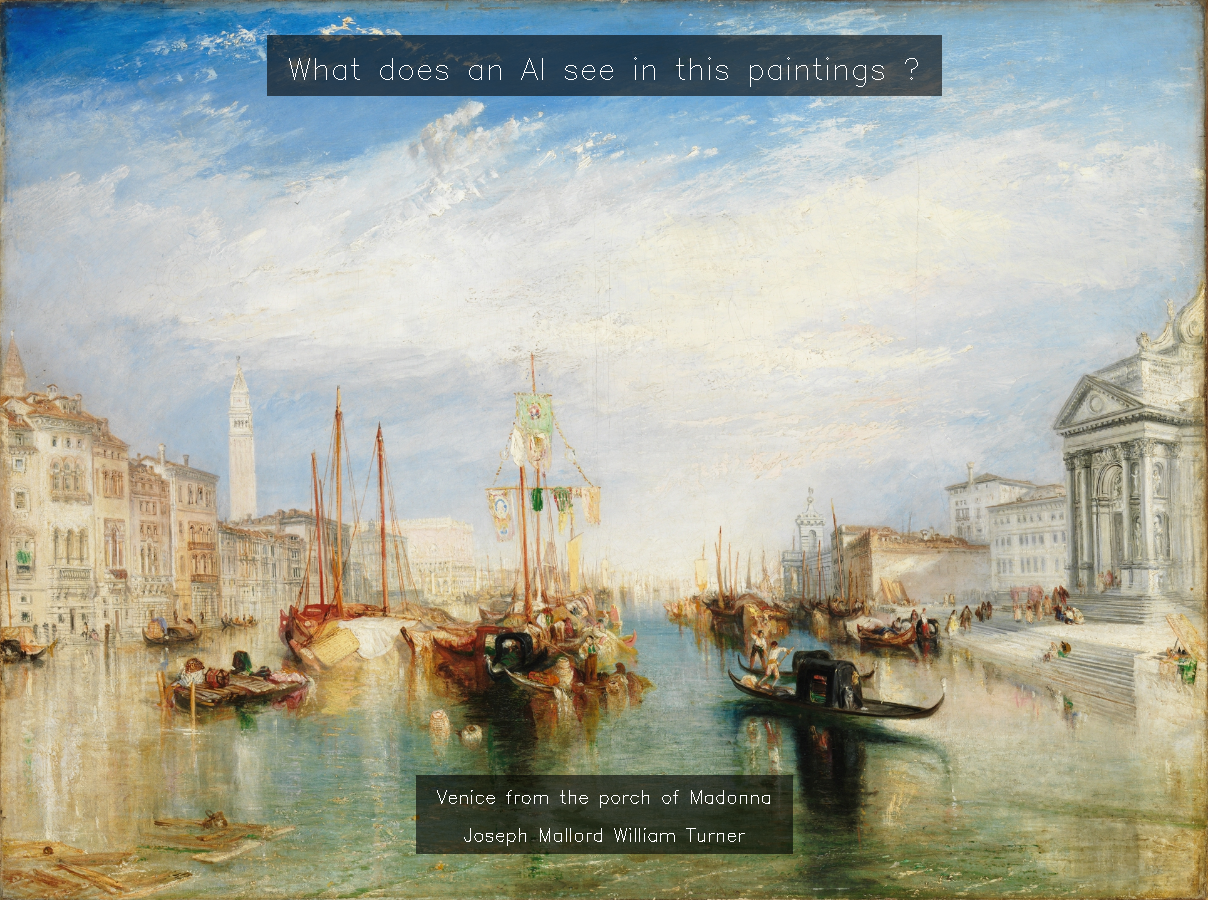
\includegraphics[width=0.7\linewidth]{datas/title_screen.png}
  \caption{Début de la vidéo (\emph{Venice from the porch of Madonna}, Turner, 1835)}
  \label{fig:title_screen}
\end{figure}

